
\documentclass{article}
\usepackage[utf8]{inputenc}
\usepackage{graphicx}
% RENAME FILE TO 910995.pdf when I submit.
\usepackage[colorlinks=true,allcolors=black]{hyperref}%
% change reference style to [1], remove stupid sorting, language changed so date in ddmmyyyy
\usepackage[backend=biber, style=numeric, sorting=none, language=australian]{biblatex}
\addbibresource{References.bib}

\title{Detecting User Engagement Using \\ Mouse Tracking Data:\\
    \large Project Specification
}
\author{David Saunders (910995)}
\date{May 2020}

\begin{document}
\maketitle

\begin{abstract} 
    This project specification reviews relevant materials and the background of my project.
    The motivation and aims of the project are explained, and a comprehensive plan of work for the summer is present.
    
\end{abstract}

\tableofcontents

\newpage

% \section*{Mark scheme}
% This coursework contributes 50\% of the mark for the module. The size is
% approximately 5000 words (excluding references) – due on Wednesday 29
% April 2020 (11:00 am).

% This report should give a literature review over your project and describe
% any background research that you have carried out. 
% You should state the motivation and aims of the project. 
% It should include a complete specification of your project. 
% It should describe the project clearly and the components
% of the work which need to be developed. 
% An outline project plan for the summer should be included. 
% This plan should take into account the development methodology being used. 
% You should provide a risk analysis for the project. 
% You should view this document as providing the plan for the work
% you expect to carry out over the summer.

% Work so far if I want?
% Anticipate what people want to see.
% NOTE IN RISKS
% done initial data analysis - has certain properties.
% ANTICIPATE AUDIENCE.

% Expand on risks if I want. Probably not in table.
% LOOK OVER M10 LECTURES. CSCM10 - CSCM10 - CSCM10 - CSCM10 - CSCM10 - CSCM10 

% COnstant reevaluation, never gonna have a perfect algorithm.

% Severity and likelihood.
% 



% TO SUMMARISE The structure POINTS
% - Literature Review
%   - Background research
% - Motivation and aims of Project
%   - Clearly describe project and components 
% - Outline Project Plan
%   - Include methodology used. 
% - Risk Analysis

% • Title
% • Abstract summarising the project
% • Introduction
%       • Motivation
%       • Aims of the project
% • Background research
% • Description of the project.
%       • Including components of the work.
% • Project plan
%       • Gantt chart
%       • Risk analysis
% • Conclusion.
% • Bibliography.

% TODO: Tom email reply

% TODO: Extend motivation lots.
% TODO: More explanation of sprints.
% TODO: Project components.

% TODO: Machine learning techniques background research.
% TODO: 'Beef up' Abstract and conclusion.

% MOTIVATION
% The motivation is probably one of the most important sections. 
% That being, I think you can extend your motivation quite a bit. 
% It's worth spending some space on why this
% problem is hard and why any obvious solutions won't work.

% GANTT CHART
% I think your gantt chart is fine, but you should give a bit more
% information about what you're going to do in the sprints themselves. 
% You can talk about things like trying different representations 
% of the data, different algorithms, etc.

% Components of project
% Ah, ok. So the different components in this case would be the 
% different things to test. This would include different
% representations of the data (aka feature sets) and different 
% algorithms. You should list the options explicitly
% (i.e. say "decision tree") rather than being vague. 


\section{Motivation}
% MOTOVATION IS WHY

%https://academia.stackexchange.com/questions/44784/how-to-explain-things-in-the-motivation-section-of-a-mathematical-paper-without
% People have wondered about how to better understand frobs ever 
% since Richard Feynman first used them to pick the locks in Los Alamos. 
% Although X, Y, and Z attempts have been made, none of them got very far
%  because they were all green-colored. 
%  In this dissertation, I examine an alternate path, reducing the problem
%   of frobs to the simpler system of greebit-space by means of an 
%   innovative application of wibbling. 
%   These results bring us one step closer to solving the problem of frobs, 
%   and how they can be better used to quickly and cheaply pick locks.

% Paragraph 1 - Initial motovation
Crowd-sourcing marketplaces like Amazon’s Mechanical Turk are popular services that provide a method for researchers to get participants to complete human intelligence tasks \cite{paolacci2010running}. 
A common use for this technology is to label data for use in training for machine learning algorithms \cite{chang2017revolt}.
However, they can also provide a cheap, scalable method for scientists to gather responses in research.
The level of user engagement, attention, and low quality responses can all be issues when gathering data from participants with distributed approaches \cite{ipeirotis2010quality}.
%Low quality answers from research projects on Amazon's Mechanical Turk are a problem - describe process.
%The primary motivation of this project is to develop a system where the mouse data of a crowdsourced user can be analysed, and from that data 
The primary motivation of this project is to develop a system of identifying if a crowdsourced user is paying attention during a task.
%For that purpose  

% Paragraph 2 - Inter disciplinary
The use of gathering responses using Amazon's Mechanical Turk and other crowdsourcing alternatives are becoming prevalent across disciplines.
It is commonly used in conducting clinical research \cite{chandler2016conducting} and it is estimated that almost half of all cognitive science research involves the use of crowdsourcing services to collect data samples \cite{stewart2017crowdsourcing}.
The creation of an easy to implement method to measure user engagement would massively help researchers to increase reliability of their research.
%If researchers user engagement can be qualified it would help to increase reliability of research.

% Paragraph 3 - Motivation
Research has been conducted on how the accuracy and attention of crowdsourced tasks can be increased.
% Look at these papers to see how they classified attentions.
Methods such as offering financial incentives \cite{ho2015incentivizing} and engaging a users curiosity \cite{law2016curiosity} have been found to motivate workers into performing better at crowdsourced tasks.
Despite the research there is still debate as to which method is superior.
If user engagement can be effectively identified then the best method of ensuring user engagement could be found using this method.

% Paragraph 4 - Why measuring attention is hard and why obvious solutions wont work. 
% It's worth spending some space on why this problem is hard and why any obvious solutions won't work

%Maybe it is hard to quantify attention as it is hard to do so.
%Measuring attention is hard and obvious solutions wont work.
Measuring user engagement is well studied in the field of web analytics \cite{peterson2008measuring}.
However the existing methods of reporting and analysing website data cannot be easily applied to crowdsourced tasks.    
Characteristics such as session duration and customer satisfaction are used as proxies for engagement.
However a longer session doesn't necessarily mean a more engagement user and customer satisfaction is not applicable for crowdsourced tasks.
Therefore existing solutions will not work and now methods must be evolved.

% TODO: ACTUALLY ADD DONT JUST IGNORE
% TODO: In the first sentence say how crowd sourcing is traditionally been used for tasks such as labelling image datasets for machine learning training data.  
% TODO: However recently scientists have become aware of the advantages crowdsourcing can have (high number ) when used to gather responses for scientific surveys.
% Theyre even being used in the fight against Coronavirus

% People are lazy. 
% Often don't pay much attention 
% Is there any way of measuring people's attention?

% Why mouse data?
% Mouse cursor position is strongly correlated with eye position. 
% One paper calls it a “poor man's eye-tracker” [find]
% Bulky expensive equipment for eye tracking is expensive and very obtrusive.
% Hawthorn / observer effect - People react differently when being observed. 
% Less obtrusive mouse tracking can make people feel less tracked and act more naturally. % goecks2000learning talks about unobtrusively observing people. CITE/TALK ABOUT 
% Could even not tell them (legal ethical repercussions)!


\section{Introduction}
%Can copy from presentation slides but fill in so they're more wordy.
% INTRODUCTION IS WHAT

This project uses data from a previous study where participants were asked to perform a simple repetitive tasks \cite{tom2018risk}.
Data was gathered both with a closely monitored lab study, and using a crowd-sourcing website.
We assume that participants in the lab study were paying attention, and that crowd sourced participants may or may not be paying attention.
The task of this project is to classify crowdsourced participants to determine who were paying attention during the task.
We hypothesise that a participants level of attention can be measured from their mouse movement data.
The project will propose methods of identifying and quantifying user engagement by using machine learning and visual analytics techniques.


\begin{figure}[ht]
    \centering
    \centerline{
        \frame{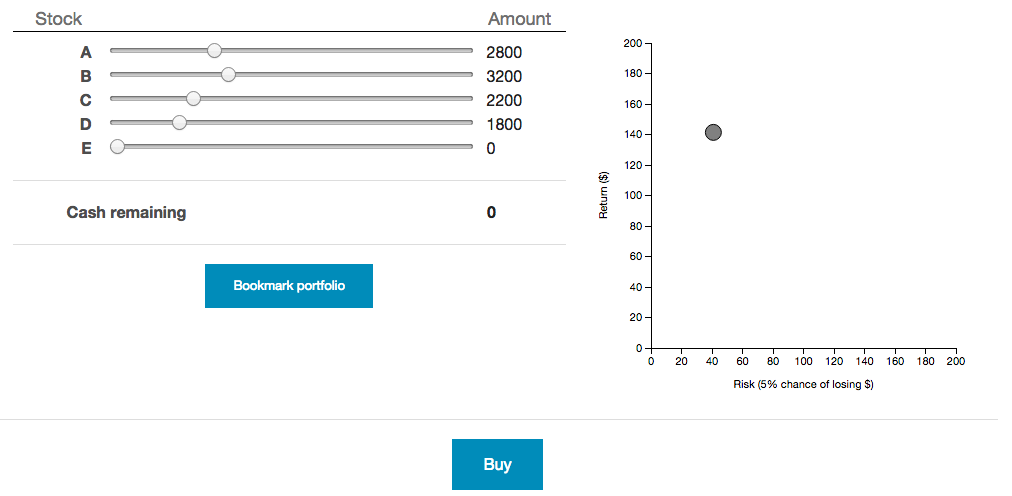
\includegraphics[scale=0.45]{interface.png}}
    }
    \caption{The user interface for the study \cite{tom2018risk}.}
    \label{fig:interface}
\end{figure}

Fig \ref{fig:interface} is the design of the interface participants of the study interacted with.
THe study modelled an investment scenario where participants were asked to maximise profit made over a series of steps.
Participants may interact with the stocks sliders to select how much of a stock they would like to buy.
The return and risk is shown on the plot on the right of the figure, this plot updates when the sliders are changed in an attempt to inform participants of the stocks volatility.
It is hypothesised that participants paying more attention will interact with the sliders more attempting to find the best combination, something their mouse data may reveal.

\begin{table}[ht]
    \caption{\label{table:studies} Data collection methods used in the study \cite{tom2018risk}.}
    \small
    \begin{tabular}{lll}
        \hline
        Data collection method & Number of participants & Were participants paying attention? \\    \hline
        Lab study              & 18                     & Yes                                 \\
        Crowdsourced task      & 370                    & Unknown                             \\    \hline
    \end{tabular}
\end{table}

Table \ref{table:studies} shows the two different ways in which data was collected.
Only 4.6\% of the data was gathered in person, with the vast majority of responses being crowdsourced.
The difference in number of participants shows one of the reasons crowdsourcing is popular. 
It is much easier to crowdsource responses than it is to organise an in person lab study.


\subsection{Aims of project}

The aims of what I want to achieve in the project will be as follows:
\begin{itemize}
    \item Visualise, analyse and understand the data.   % data from the previous study
    \item Use the data to train machine learning models to classify users by their attention level.
    \item Determine if there is a link between a users attention and task performance.
    \item Combine the data and methods from the study data with other crowdsourced datasets to create a more robust model.
    \item Publicly share all data and findings of this project.
    %\item Test any methods and models developed with other applications?
\end{itemize}

Here I detail how I will achieve each aim, and describe the components of the project that I will need to complete.
% Try and link each component of the project to an aim.

To visualise and understand the data I will use tools like Tableau to create basic plots such as histograms.
If any interesting correlation or information is found in the data at this stage it can be more fully explored in depth later in the project.

% Any correlations found here can be explored in depth later.

Semi supervised learning techniques can be used to classify which of the crowdsourced participants were paying attention.
The idea of semi-supervised learning is combining labelled and unlabelled data to improve the learning behaviour of a machine learning technique \cite{zhu2009introduction}.
This will be used in this project as only a subset of the data is labelled, where the lab study results are labelled as paying attention and crowdsourced results are unlabelled.

To see if a users attention influences their task performance relies on me being able to extract user attention information from the mouse data.
If I am unable to do so I could attempt to use just the lab study data, however there is only a small number of datapoints, and not enough to make a significant


Other datasets can be researched and explored.
Similar datasets do exist online and are publicly available \cite{kaggleWorkerActivity}.
Overfitting is a big issue with any machine learning technique, especially when there is not a large amount of data for training \cite{dietterich1995overfitting}.
In an attempt to avoid this I can increase the quantity of data available to me by incorporating other sources and hopefully create a more robust model.
% Applications
% A good system developed could be used for other tasks to monitor attention - E.g. Survey Monika made us do. Not just for joes ice-cream
% Have to decide on the trade off between a good narrow (is this the right word) classifier between attention or not and a more generalised model that can work on any task.
% What I mean by that is I can model the html elements / sliders to see how users interacted to see the stock prices, or I can generalise to any such task involving mouse data.



To publicly share the result of this project I will upload any work completed for it in a GitHub repository.
Sharing data and results with the Data Science community is an important part of scientific research as it allow others to peer review and reproduce my results \cite{Birnholtz2003data}.

% Machine learning methods
%     SVM
%     Natural Language Processing
%     N-Grams
%     LSTM Neural Networks
%     Markov models
% Deal with Imbalances in classes
%     Sampling
%     Oversampling, Undersampling
% Other mouse data sources


\section{Background Research}

% Anything I've looked at with help for mouse data classification algorithms? 
% %\section{Literature review}
% In this section I will review the literature on how to monitor attention.
% %This can pretty much be the review I did for the first assignment. 

I have introduced the background as to why it is important to detect user engagement.
Now the existing literature will be examined to see how others have proposed to solve this problems and explore any methods that may be used in this project.


% \subsection{User attention and characteristic.}

% If I think of anything good to write put it here, else delete section.

% Dont really link to engagement 
\subsection{Eye tracking}

Non-verbal information such as eye tracking may be used to detect user’s level of engagement \cite{lala2017detection}.
Vision is one of the most powerful human senses so it has the potential to give a good measure of user engagement. 
The methodology of eye tracking is that we move our eyes to focus on particular areas that we want to see in more detail, and divert our attention to that area \cite{duchowski2007eye}. 
% duchowski2007eye is a VERY important piece of literature for the field, over 4000 citations
Thus tracking a user’s gaze can provide insight into which part of a system they’re engaged with, and how much so.

\begin{figure}[ht!]
    \centering
    \centerline{
        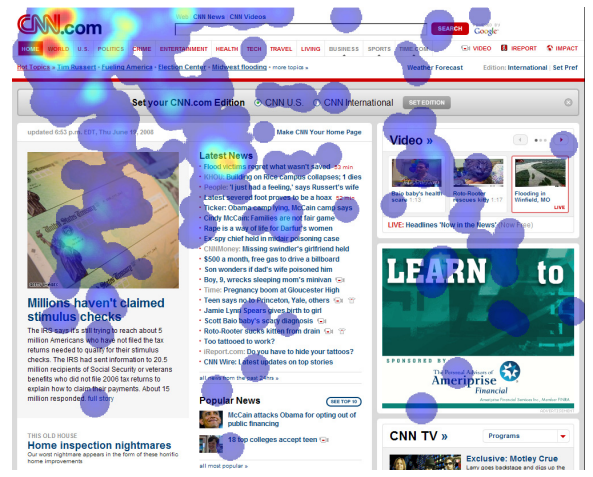
\includegraphics[scale=0.85]{EyeHeatmap.PNG}
    }
    \caption{Heatmap showing popular locations of users eyes on a webpage \cite{buscher2009you}.}
    \label{fig:eyetrack}
\end{figure}

Eye tracking data can be used to show user interface elements that users focus their attention on as shown in Fig \ref{fig:eyetrack}. 
From this researchers were able to predict the amount of attention elements of the page would receive.
By observing what parts of an interface users are interacting with we can determine what a user is engaging with \cite{buscher2009you}.
Eye-tracking has been used, and found success novel applications such as recording the engagement of users when playing a game. 
Tracking users eye movements helped game designers understand how users can recognise interactable game objects and could be used to investigate problematic game design issues \cite{renshaw2009towards}.

Eivazi and Bednarik extracted features from a users eye tracking data to determine their cognitive state in a problem solving exercise \cite{eivazi2011predicting}.
Features such as ``mean fixation duration'' and ``total path distances'' were engineered, and users were split into classes based on their performance. 
Given a user feature set and their performance class it was able to classify their cognitive state during the task with a 87.5\% accuracy with a support vector machine.

Szafir and Mutlu identified a plethora of verbal and non-verbal behavioural cues used by teachers in an educational setting, with gaze being identified as one of them \cite{szafir2012pay}.
The behavioural cues could not be recorded directly by a computer, instead EEG signals measured from a headset were used to measure engagement.

Eye tracking is not however a perfect solution and its limitations have been well documented. 
Track subjects eyes with a good degree of accuracy requires the use of expensive, intrusive equipment that frequently needed recalibrating \cite{richardson2004eye}. 


\subsection{Mouse cursor tracking}
% Copied straight from CSCM10 Initial Report
% Mouse cursor tracking

Research has also found that there is a correlation between a user’s gaze and their cursor position. 
The position can be considered a ``poor man’s eye tracker'' as it has been found that eye gaze match mouse position 69\% of the time \cite{cooke2006mouse}. 
Mouse movement data can be collected without the drawbacks of eye tracking and with more automatic methods, meaning more data can be collected, and on a larger scale \cite{demvsar2017quantifying}.
Therefore it can be said that mouse data can be used as a good alternative to eye tracking data.

%Mouse activity can be used as input to a neural network and output a quantifiable level of activity for a webpage. 
By using mouse data it is possible to unobtrusively record a user’s normal use of a web browser without disturbing their experience \cite{goecks2000learning}.
% Above paper touches on one of the big advantages of measuring user engagement from mouse data, it is unobtrusive! We can monitior them in the background 
It has also been found that users tend to follow the text they are reading with the mouse cursor \cite{liu2007detecting}. 
It can be determine what paragraph of a page was being read with an accuracy of 79\% by using mouse cursor data \cite{hauger2011using}. 

Other methodologies explored ways of classifying user engagement from eye and cursor data, however it is also possible to predict users attention and user frustration in complex webpages \cite{navalpakkam2012mouse}.
Not all studies agree that mouse cursor is always a good approximation for eye data. 
Hauger et al found that distinct cursor behaviour exists depending on the task, and that the relationship between eye gaze and mouse position is more nuanced than measuring only mouse data \cite{huang2012user}.

% \subsection{Machine learning techniques}
% I've given a high level overview of the existing literature, here I will be more in depth as to the algorithms and techniques relevant to this project.

% Machine learning methods
%     SVM,
%     Natural Language Processing,
%     \underline{N-Grams},
%     LSTM Neural Networks,
%     Markov models,
% Deal with Imbalances in classes,
%     Sampling,
%     Oversampling, Undersampling

% Machine learning has been used before to measure user engagement and interface interaction.
% Langly developed a method in which machine learning was used to create a modified user interface for users that they interact with the best \cite{langley1997machine}.




\subsection{Text classification}

Text classification is an increasingly popular task in the field of data mining.
This typically involves labelling a document into categories by analysing their text content.
Examples of this include new filtering where articles are assigned a category or spam filtering where emails can be classified as spam \cite{aggarwal2012survey}.

Nigam et al shows how a the use of Expectation-Maximization and naive Bayes classifier can be used to classify text documents into categories by looking at the distribution of words in a document \cite{nigam2000text}.
% Add sentence explaining method more
A classifier is trained on labelled data which is then used to label unlabelled data.
This method of combining supervised and unsupervised learning was found to work better than solely using labelled data.
This is especially important with text classification as unlabelled data is much more plentiful than labelled data.

In this paper a document is defined as an ``ordered list of word events'', however their approach could be applied to other forms of data.
We can define a users mouse data as an ordered lists of mouse events.
Therefore a similar approach could be used in this project where the frequencies of mouse events are recorded and used in combination with a classification algorithm.

\subsubsection{N-Grams}

The method by Nigam et al would be considered an unigram model of natural language processing.
An n-grams is a series of n words, with unigrams being one word, and bigrams being two word pairs \cite{keselj2009speech}.

Different n-grams can be combined together to better understand the complexities of a text document.
A mixture of unigrams, bigrams, and trigrams can extract different levels of text complexity and perform well with document classification \cite{aggarwal2012survey}.


% \subsection{Dealing with unbalanced classes}

% The purpose of crowdsourcing responses is to increase the number of participants in the study in an attempt to get a wider spread of data without bias.
% As a result there are many more crowdsourced responses than lab study responses, as shown in Table \ref{table:studies}.
% The sparseness of samples definitely paying attention leads to massive imbalances in the number of samples between tasks.
% \url{http://citeseerx.ist.psu.edu/viewdoc/download?doi=10.1.1.43.4487&rep=rep1&type=pdf}


% \url{https://towardsdatascience.com/methods-for-dealing-with-imbalanced-data-5b761be45a18}




\section{Description of the project}

The high level aims of the project have been given, this section will more concretely detail what work must be done. 

\subsection{Components of project}

The component's can be separated into individual sections, however there is still an order that they must be completed in.

% MEG says to delete.
%Now that the background for the project has been researched the more technical programming side of the project can begin.
The data must first be extracted from the JSON format that its in to a more tabular format.
The project will then consist of researching different algorithms and methods and attempting to implement them on the project data.

Different methods of data extraction or feature engineering may be explored.
Any results from this will then be analysed, visualised, and evaluated.
These stages can be repeated multiple times as different methods are explored.
After multiple different approaches have been explored the results should be properly documented and compiled in my dissertation.

% Ah, ok. So the different components in this case would be the different
% things to test. This would include different representations of the data
% (aka feature sets) and different algorithms. You should list the options
% explicitly (i.e. say "decision tree") rather than being vague. 

Feature engineering can be approached in a similar was as Eivazi and Bednarik \cite{eivazi2011predicting}.
Features such as total time, time for each step, total mouse distance, mouse movement speed, and time spend on different elements can be extracted.
Each of these may be systematically investigated, modified, and evaluated until useful data is engineered.
If there is too much variance between users I can attempt to split them into groups based on their task performance.
A certain combination of features may revel attention levels in the badly performing group but the approach may not be successful with the well performing group. 

The purpose of crowdsourcing responses is to increase the number of participants in the study in an attempt to get a wider spread of data without bias.
As a result there are many more crowdsourced responses than lab study responses, as shown in Table \ref{table:studies}.
Therefore methods of dealing with data with imbalanced classes are another component of work that must be completed. 
If this is not addressed the the sparseness of data from users definitely engaged in the task may lead to erroneous results when classifying crowdsourced data \cite{kubat1997addressing}.
The sampling methods of over and under sampling data can solve this problem.
Oversampling is where new data are created from the sparse class and with undersampling data is removed from the abundant class \cite{drummond2003c4}.

% Ladder networks are one method of semi-supervised learning.
% https://rinuboney.github.io/2016/01/19/ladder-network.html

%TODO: Look at the dissertation outline so I know what stuff needs to be included so I can mention it here.

\subsection{Description of data}

The first component of the project has been completed, and data has been extracted form JSON format to a csv format.

\begin{table}[ht]
    \caption{\label{table:data} The first 5 records of results of the crowdsourced task.}

    \begin{tabular}{llllllll}
        \hline
        event\_type    & target         & time  & x   & y   & step & turkId         \\ \hline
        mousedown      & alloc-slider-1 & 0     & 477 & 405 & 1    & A35YFAFWP33C70 \\
        mouseup        & alloc-slider-1 & 0.111 & 478 & 405 & 1    & A35YFAFWP33C70 \\
        click          & alloc-slider-1 & 0.111 & 478 & 405 & 1    & A35YFAFWP33C70 \\
        mousedown      & alloc-slider-1 & 1.516 & 479 & 405 & 1    & A35YFAFWP33C70 \\
        mousedirchange & alloc-slider-1 & 2.395 & 543 & 403 & 1    & A35YFAFWP33C70 \\
        mousedirchange & alloc-slider-1 & 3.161 & 594 & 402 & 1    & A35YFAFWP33C70 \\
        mouseup        & alloc-slider-1 & 5.048 & 514 & 407 & 1    & A35YFAFWP33C70 \\
        click          & alloc-slider-1 & 5.048 & 514 & 407 & 1    & A35YFAFWP33C70 \\
        mousedown      & alloc-slider-2 & 5.461 & 494 & 441 & 1    & A35YFAFWP33C70 \\
        mouseup        & alloc-slider-2 & 5.513 & 494 & 441 & 1    & A35YFAFWP33C70 \\ \hline
    \end{tabular}
\end{table}

Table \ref{table:data} shows us the features of the data.
The lab study data and the crowdsourced data have the same schema, except lab results have a different ID field.

The target field shows us which element in Fig \ref{fig:interface} a participant is interacting with and event\_type details the type of interaction.
Time field shows the time taken in seconds since the first recorded mouse event.
We can hypothesise that participants with a shorter time paid less attention than a participant who took much longer, thinking about their actions more.
The x and y fields show the location of the mouse and step shows which stage of the task, from 1 to 5, a participant was in.


\section{Project plan}
% Look into different software methodologies
% http://www.cs.swan.ac.uk/~csetzer/articles/researchMethodologiesInComputerScience.pdf
% 

The different components of the work have been explained above.
This section will specify the timeframe and the order in which the modules will be carried out.

\subsection{Development methodology}
%Discuss software life cycle methodologies with Jacques.
% An agile methodology such as scrum would probably be best but am I constrained  by this specification document?

% We want a methodology that has a final write up, but also has lots of iterative stuff in the middle for me to research, explore, and test new algorithms.
% For that reason I will be following the Scrum software lifecycle methodology.
% TODO: reference 

% Give a breif explaination of Agile.

I will be using an agile methodology as it will allow flexibility of my project and the iterative nature should help me to constantly improve it \cite{beck2001manifesto}. 
Scrum will be used as the short scrum periods will encourage bursts of development over the long summer period \cite{schwaber1997scrum}.

\begin{figure}[ht]
    \centering
    \centerline{
        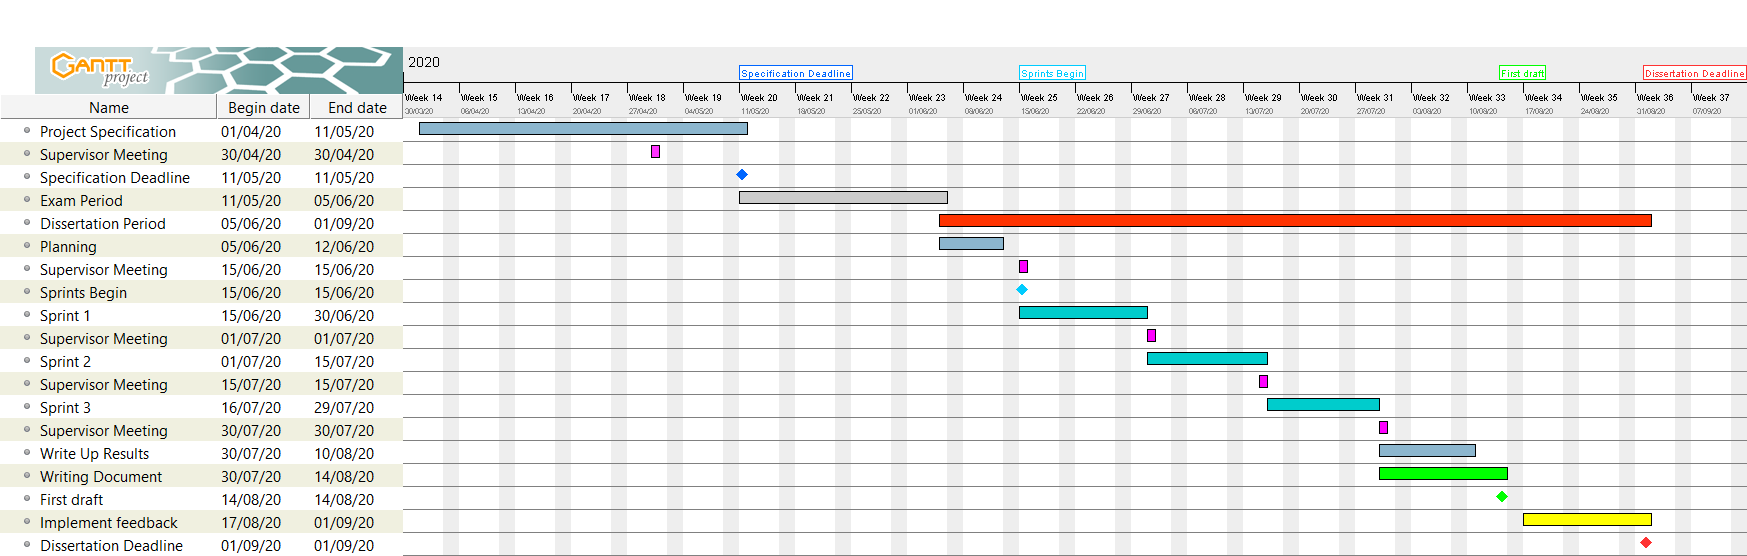
\includegraphics[scale=0.32]{GanttChart.PNG}
    }
    \caption{Gantt chart showing the planned timeline and milestones of the project.}
    \label{fig:Gantt}
\end{figure}

Fig \ref{fig:Gantt} shows the sprints I will be undertaking.
The Gantt Chart was created with the free software Gantt Project \cite{GanttProject}.

A sprint will begin with a supervisor meeting where the previous work, and the plan for the next sprint will be discussed.
There will be three sprints in total, with each sprint being a fortnight long.
Each sprint will consist of researching a method such as a certain machine learning algorithm or different feature engineering techniques I may be able to use in my project.

Time will be spent modifying and implementing the method so that it may be used in the context of this project.
The latter half of a sprint will consist of analysing and visualising the results of the method and writing these down roughly in the dissertation document.

The effectiveness of the method will be evaluated and I will attempt to fix any failures or shortcomings of the method.
For example I may research variants of artificial neural networks that show promising potential.
The sprint plan would allow me to spend time implementing this network with my data and experiment with the parameters.  


% TODO: Implement Toms email feedback
% I think your gantt chart is fine, but you should give a bit more
% information about what you're going to do in the sprints themselves. You
% can talk about things like trying different representations of the data,
% different algorithms, etc.


\subsection{Risk analysis}
% Copy risk analysis from last year.
When creating a project there is always potential risks that the project might encounter and hinder its chances of success. 
In order to prepare and to hopefully avoid these risks I will now list and analyse the risks of my project.

Each risk is explained with the likelihood of the risk occurring and impact to the project the risk would have.
A mitigation plan is created in an attempt to prevent the risk from happening, and a contingency plan is made so I can be prepared if the risk does occur.
The likelihood of a risk occurring is measured from low to high.
Low likelihood risks are unlikely to happen and high is very probable to happen. 
Impact is measured on the same scale.
A low impact risk will have little influence, where as a high project would massively effect it.
Below I have listed and analysed the risks and have ordered them from potentially the most dangerous to least dangerous. 

% TODO: Flesh out risks 

\begin{enumerate}
    \item 
    \begin{description}
        \item[Risk:]    
        \emph{Unrealistic time plan and poor time management.}
        \item[Likelihood and Impact:]
        Medium likelihood, Medium Impact
        \item[Explaination]
        If my time is spent poorly then I could not have a piece of work finished for the submission deadline, or the work may not represent the best of my abilities.  
        \item[Mitigation:]
        Create work schedule and stick to it.
        A work schedule and plan for the summer has been created in this document which I aim to follow.
        \item[Contingency:]
        If I am unable to stick to my work schedule, I must adapt my approach to work and create an undated, more realistic schedule.
    \end{description}

    \item 
    \begin{description}
        \item[Risk:]
        \emph{Coronavirus affects me or a close family member, negatively effecting my work.}
        \item[Likelihood and Impact:]
        Medium likelihood, High Risk
        \item[Explaination]
        Coronavirus is very contagious. 
        In spite of protective measures it is still likely that I may become infected with the virus. 
        \item[Mitigation:]
        Stay safe indoors during the quarantine to keep everyone safe and mitigate any risks of me becoming infected.
        \item[Contingency:]
        Inform the University as soon as any negatively situation develops so that alternative assessments can be organised.
    \end{description}

    \item 
    \begin{description}
        \item[Risk:]    % TODO: Emphasise I mean in the data and not at all?
        \emph{No correlation between attention and mouse tracking data can be found.}    
        \item[Likelihood and Impact:]
        Medium likelihood, High impact
        \item[Explaination:]
        The project will involve the use of many methods to find a link between mouse tracking data and user attention.
        However the number of total data samples are in the hundreds so there is not a massive amount of information to draw conclusions from.
        It is possible that after all methods have been exhausted no correlation is ever discovered, or simply doesn't exist. 
        \item[Mitigation:]
        Attempt as many different methods of classification early before writing in depth about them.  
        \item[Contingency:]
        If no insights can be gained from the given dataset, I will explore other similar datasets and attempt to find correlations there.
        I will then attempt to apply findings from other datasets to the original dataset. 
    \end{description}

    \item 
    \begin{description}
        \item[Risk:]    
        \emph{Coronavirus has a greater impact on Swansea University and effects my available support and deadlines.}
        \item[Likelihood and Impact:]
        Low likelihood, Low impact
        \item[Explaination:]
        The virus has already shut down in person teaching and with the UK in lockdown it is unlikely the situation will become vastly different. 
        \item[Mitigation:]
        Keep informed with the University College of Science and supervisor to any news effecting the University.
        \item[Contingency:]
        Keep updated with the situation and follow whatever advice is recommended from the university.
    \end{description}

    % TO ADD ANOTHER RISK IF NECESSARY
    % \item 
    % \begin{description}
    %     \item[Risk:]    
    %     \item[Likelihood and Impact:]
    %     \item[Mitigation:]
    %     \item[Contingency:]
    % \end{description}
\end{enumerate}

% OLD TABLE INCASE I WANT TO REVERT
% \newpage
% \begin{table}[ht]
%     \small %small not needed
%     \caption{\label{table:individual} The top association rules between individual items.}
%     \makebox[\textwidth][c]{%
%         \begin{tabular}{|p{2cm}|p{1cm}|p{1cm}|p{1cm}|p{2cm}|p{2cm}|}
%             \hline 
%             { Risk}                                                                                                       & { Probability} & { Impact} & { Combined Risk} & { Mitigation Plan}                                                                                               & { Contingency Plan}                                                                                                                  \\
%             { Unrealistic time   plan and poor time management.}                                                          & { High}        & { High}   & { High}          & { Create work   schedule and stick to it.}                                                                       & { If I am unable to   stick to my work schedule, I must adapt my approach to work and create an   undated, more realistic schedule.} \\
%             { Coronavirus affects me or a close family member, negatively effecting my work.}                           & { Medium}      & { High}   & { High}          & { Stay   safe during the quarantine to keep everyone safe and mitigate any risks of me   catching anything.}     & { Inform   the University as soon as a situation develops so we can arrange something.}                                              \\
%             { Coronavirus has a greater impact on Swansea University and  effects the available support and deadlines.} & { Medium}      & { High}   & { Medium}        & { Keep   informed with the University College of Science and supervisor to any news   effecting the University.} & { Keep my   options open? Keep updated?}                                                                                             \\
%             { No correlation between attention and mouse tracking data can be found.}                                   & { Low}         & { High}   & { Medium}        & { Attempt   as many different methods of classification early before writing in depth about   them.}             & { If no   insights can be gained from the given dataset, I will attempt to find   correlations in other datasets.}                   \\                                                                                                                    
%         \end{tabular}
%     }
% \end{table}

\section{Conclusion}

% Measuring user engagement is challenging
% Mouse data can help us solve that issue by showing user attention
% Data Science techniques could be used to help classify the data (Not SVM)



% End with something nicer

% TODO make work
% The background of the project has been presented, and existing methods researched.
%This report has given an introduction to the work that will be conducted over the next few months.
In this report the motivation of why there is a need to detect user engagement in increasingly popular crowdsourcing services.
%The backgroud of the project is given  mouse tracking data may be used to do so.
The problem of detecting user engagement in crowdsourced responses has been explained and the need for a new solution is outlined.

The existing methods of eye, and mouse tracking have been researched.
It was found that mouse data has many of the benefits of eye tracking data with none of the drawbacks, making it ideal for use in user engagement.
% TODO: Add something about n-grams

A detailed plan of the project was shown, with a detailed breakdown of the timeline, and components of the project shown with a Gantt chart.
Risk analysis of the project was completed so that no unexpected incident will disrupt the project.

\printbibliography

\end{document}

% This report should give a literature review over your project and describe
% any background research that you have carried out. 
% You should state the motivation and aims of the project. 
% It should include a complete specification of your project. 
% It should describe the project clearly and the components
% of the work which need to be developed. 
% An outline project plan for the summer should be included. 
% This plan should take into account the development methodology being used. 
% You should provide a risk analysis for the project. 
% You should view this document as providing the plan for the work
% you expect to carry out over the summer.


% Project meeting
% ############## Programming Questions ############
% Points start and end at different points, for both lab and actual, is that expected? 
%     How was it measured? Moving window?
%     How do I reference this in diss?
%     Can I just transform points to new position? But how do I do other points not just start end.

% In Data online turk has alloc-slider-5 while lab study has stuff like [id="alloc-slider-return-4"]>svg>g>circle and [id="alloc-slider-return-4"]>svg. can just remove the brackets but whats the >svg>g>circle?

% Lab has no buttons,  and some that say just html?

% Presentation Questions
% #############################################

% Marks for Presentation 65 I was happy with. Feel like 65 is good a merit but lower than other marks so should I be disappointed?

% For motivation and background of project do I just say what I did in my presentation?
% onje sentence explaion what i do why and helpful. By end of first paragraph! so people dont get lost.
% Said how I will evaluate.-  we will evalutate teh algorithm by comparing again stest dataset.

% http://pages.cs.wisc.edu/~gleicher/Web/Advice/PaperRecipe

% ##################### Project Specification #################

% No existing work section on project specificaton, so I dont say anything? Not that ive done much but transform Data and do SVM.

% Literature review for project, is this not just what I did for the initial thing? cant remember what it was called but whatever.
% - Why cant trhie approach be used for mine
% Do want to add a section maybe on NLP and semi-supervised learning. But hows NLP a literature review of project, even assuming it works at all??

% In risk assessment of project, ive said covid effecting uni, and covid effecting me. 2 more risks of me failing at time management and me failing to find any correlation between mouse and attention in the data. Is this ok?

% How would I mitigate these risks?
% I think no correlation is kinda likely, while youd intuitevly think that there may be a correlation no other studies seem to back it up and with so little data points its hard to draw any actual conclusions.


% Gantt Chart

% Whole timeline.


% - Have milesstones.
% - Sub cycles 
% - initial data analysis
% - building
% - testing
% - why didnt work
% -  evaluation 
% - repeat.

